\documentclass{standalone}

\usepackage[scaled]{helvet}
\usepackage[T1]{fontenc}
\usepackage{tikz}
\usepackage{xcolor}
\usetikzlibrary{calc, positioning}

\renewcommand\familydefault{\sfdefault}
\begin{document}
  \nopagecolor
  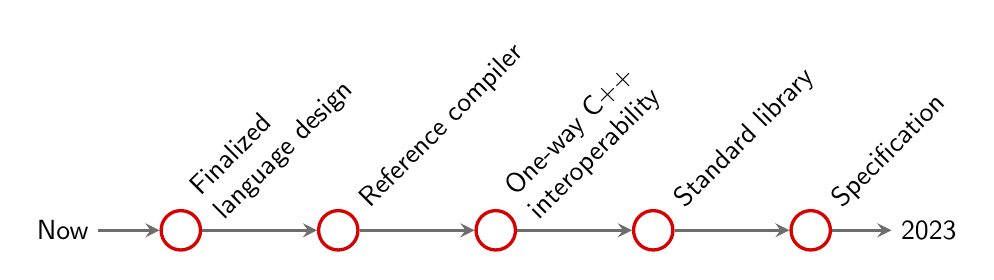
\begin{tikzpicture}
    \tikzset{
      milestone/.style={
        circle, minimum width=0.5cm, draw, very thick,
        draw={rgb,255:red,213;green,2;blue,1},
      },
      link/.style={
        -stealth, draw, very thick,
        draw={rgb,255:red,109;green,109;blue,109},
      },
      title/.style={
        rotate=45, align=left, anchor=west,
        % text={rgb,255:red,109;green,109;blue,109},
      },
    }

    \node (now) {Now};

    \node[milestone] (a) at ($(now) + (+1.5,0)$) {};
    \draw[link] (now) -- (a);
    \node[title] at ($(a) + (+0.25,+0.25)$) {Finalized\\language design};
    
    \node[milestone] (b) at ($(a) + (+2.0,0)$) {};
    \draw[link] (a) -- (b);
    \node[title] at ($(b) + (+0.25,+0.25)$) {Reference compiler};
    
    \node[milestone] (c) at ($(b) + (+2.0,0)$) {};
    \draw[link] (b) -- (c);
    \node[title] at ($(c) + (+0.25,+0.25)$) {One-way C++\\interoperability};

    \node[milestone] (d) at ($(c) + (+2.0,0)$) {};
    \draw[link] (c) -- (d);
    \node[title] at ($(d) + (+0.25,+0.25)$) {Standard library};

    \node[milestone] (e) at ($(d) + (+2.0,0)$) {};
    \draw[link] (d) -- (e);
    \node[title] at ($(e) + (+0.25,+0.25)$) {Specification};
    
    \node (2023) at ($(e) + (+1.5,0)$) {2023};
    \draw[link] (e) -- (2023);
  \end{tikzpicture}
\end{document}
